\newcommand{\dummycontentabstract}{
	\LipsumPar{75}
}

\newcommand{\dummycontentintroduction}{
	\LipsumPar{4}
	\begin{minipage}{.45\textwidth}
		\lipsum[66]	
	\end{minipage}
	\begin{minipage}{.54\textwidth}
        \begin{center}
            \includesvg[width=.8\textwidth]{./imgs/shower_example}
            \captionof{figure}{Electromagnetic shower}
        \end{center}
	\end{minipage}
}

\newcommand{\dummycontentsomething}{
	\begin{center}
		\begin{tikzpicture}
			\node (img) {
				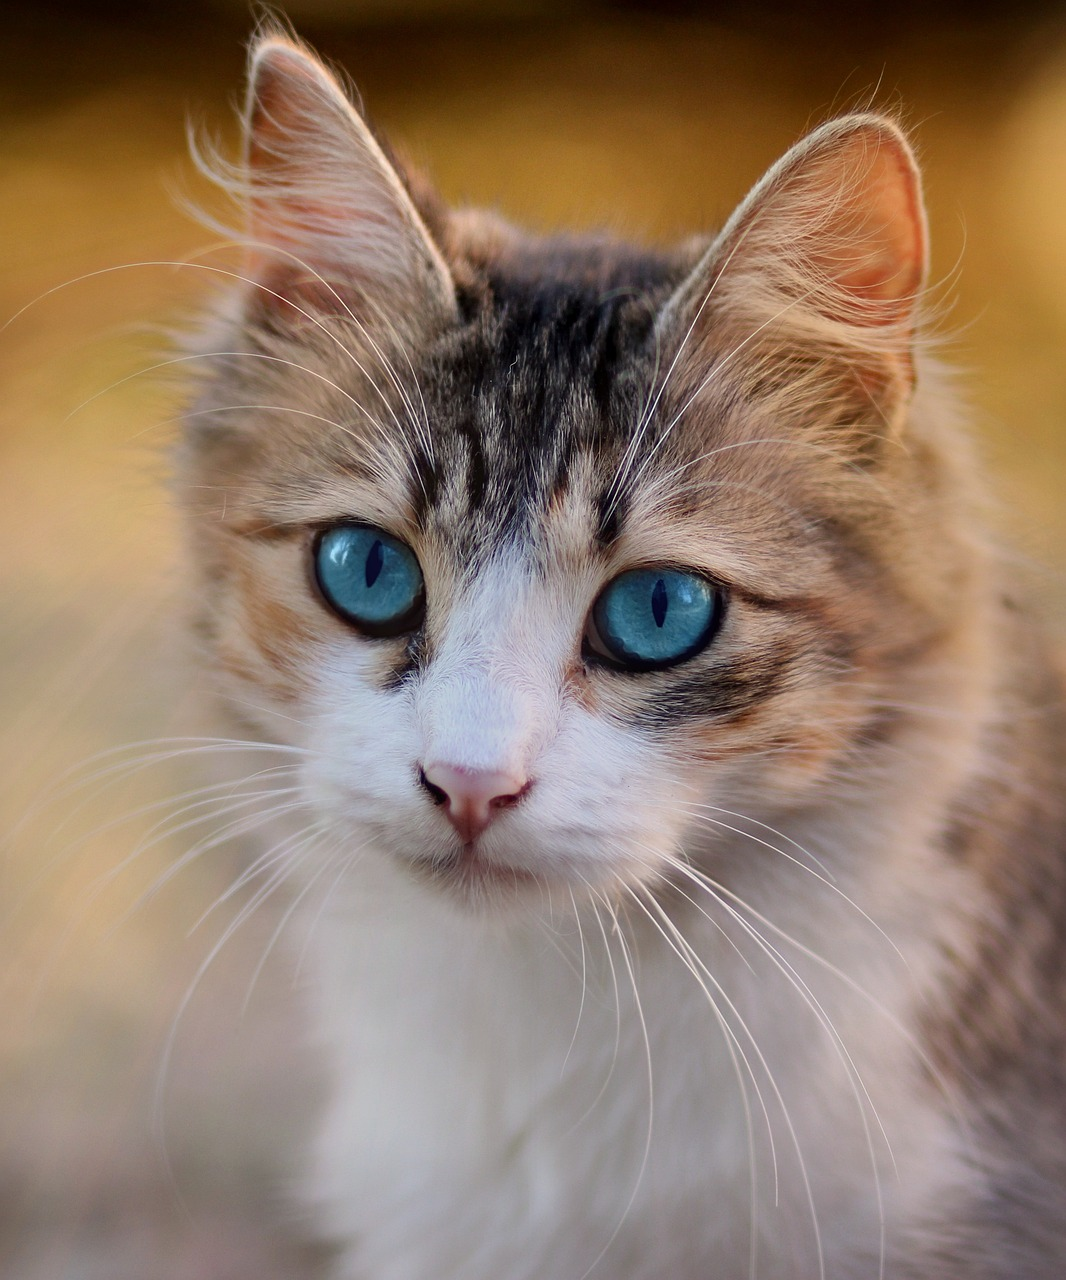
\includegraphics[width=.3\textwidth, trim={0, 5cm, 0, 2cm}, clip]{./imgs/cat.jpg}
			};
			\node (img) at (6,0) {
				\includesvg[width=.3\textwidth]{./imgs/bloch}
			};
		\draw[-{Triangle[width=30pt,length=20pt]}, line width=10pt, color=desyblue](2,0) -- (4, 0);	
		\end{tikzpicture}\\[.5cm]
		\begin{tikzpicture}
			\node (img) {
				\scalebox{1}[-1]{\includesvg[width=.3\textwidth]{./imgs/bloch}}
			};
			\node (img) at (6,0) {
				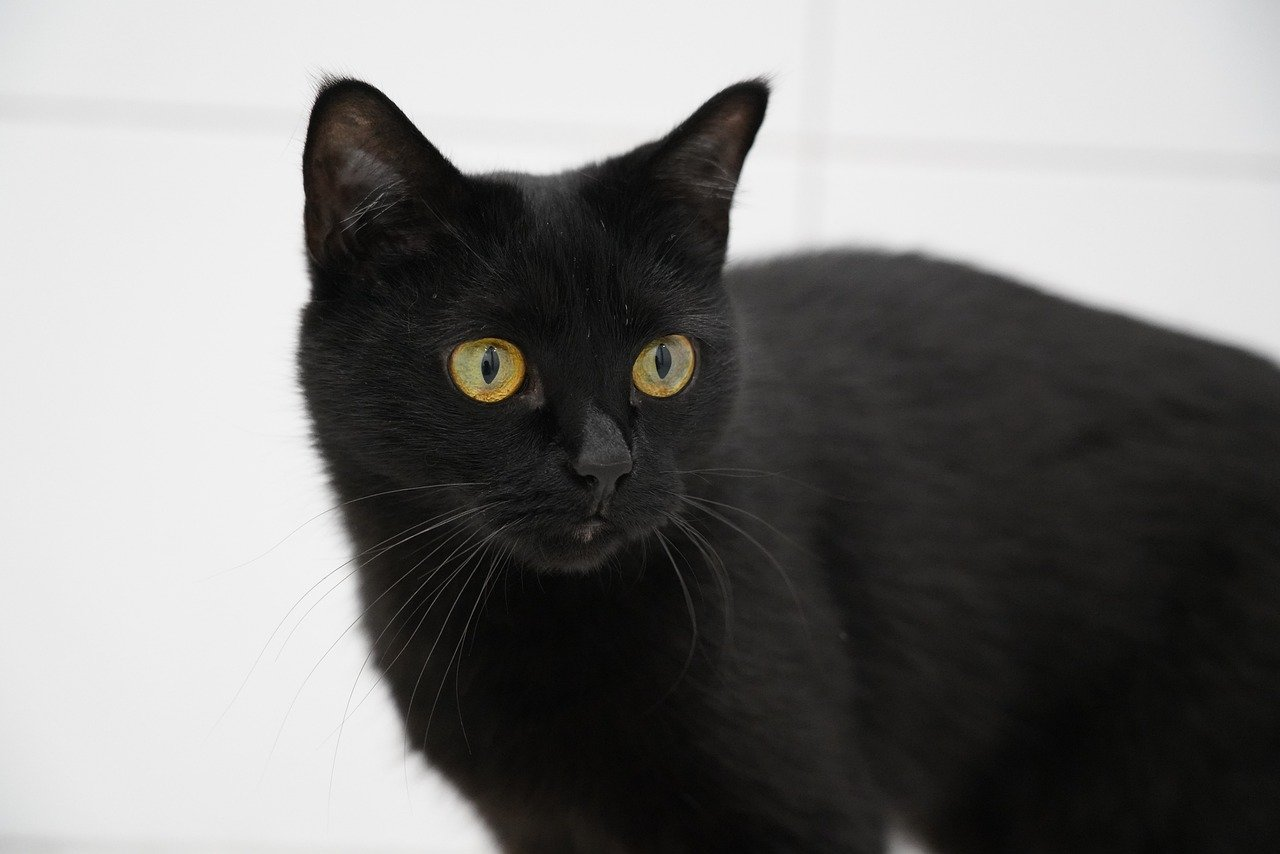
\includegraphics[width=.3\textwidth, trim={6cm, 0, 8cm, 0}, clip]{./imgs/cat_alt.jpg}
			};
		\draw[-{Triangle[width=30pt,length=20pt]}, line width=10pt, color=desyblue](2,0) -- (4, 0);	
		\end{tikzpicture}
		\captionof{figure}{A cat can be encoded into a \emph{Bloch sphere} and viceversa}
	\end{center}

	\LipsumPar{4}
}

\newcommand{\dummycontentsomethingelse}{
	\LipsumPar{4}
	\begin{center}
		\begin{tikzpicture}
			\node (img) {
				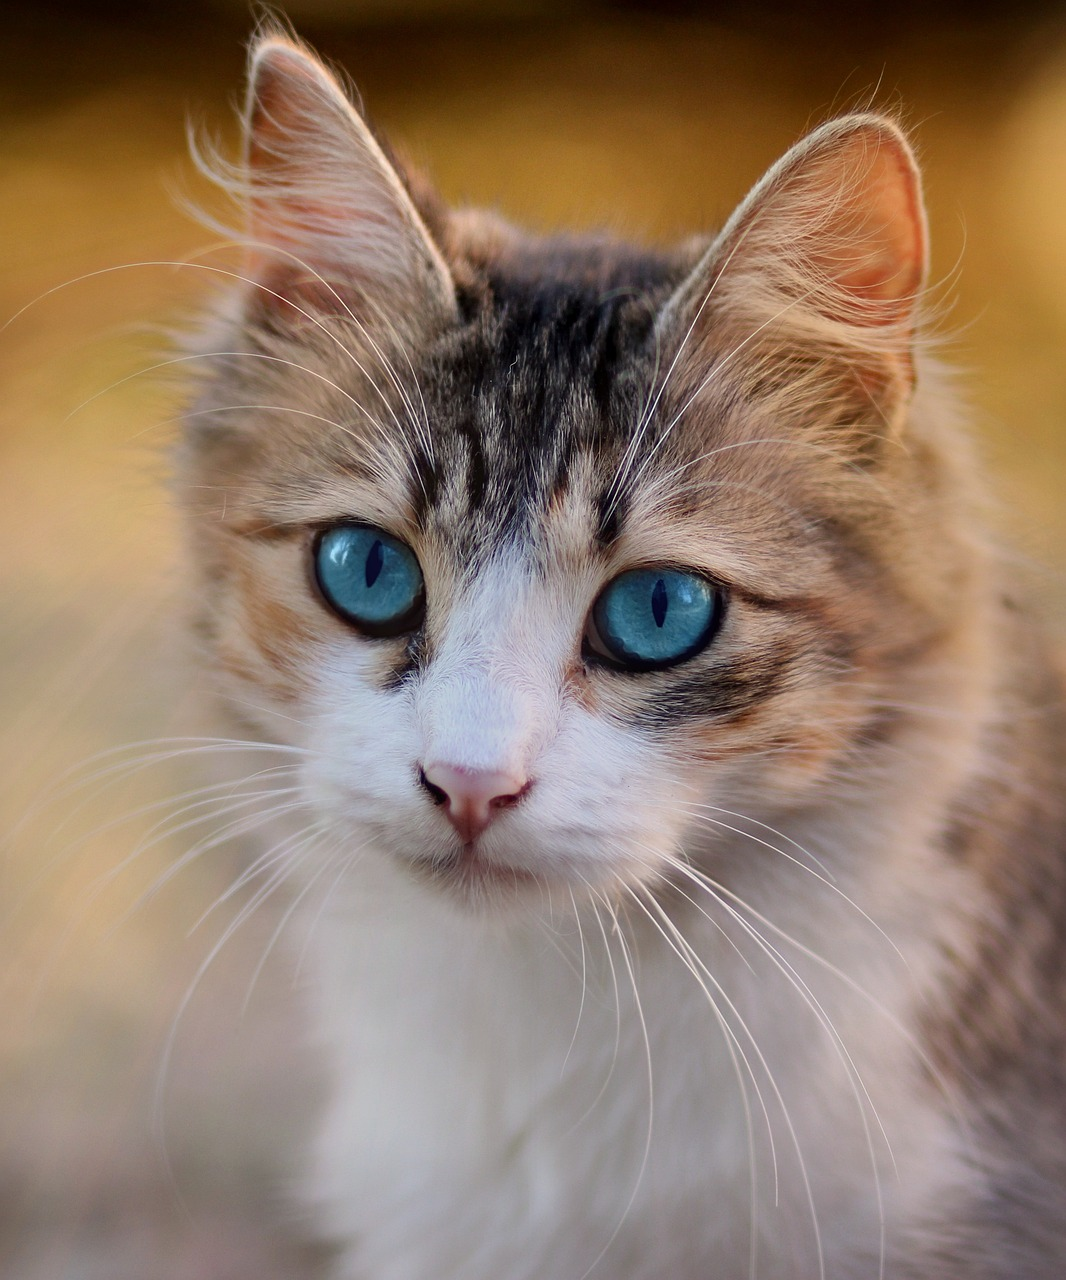
\includegraphics[width=.3\textwidth, trim={0, 5cm, 0, 2cm}, clip]{./imgs/cat.jpg}
			};
			\node (img) at (6,0) {
				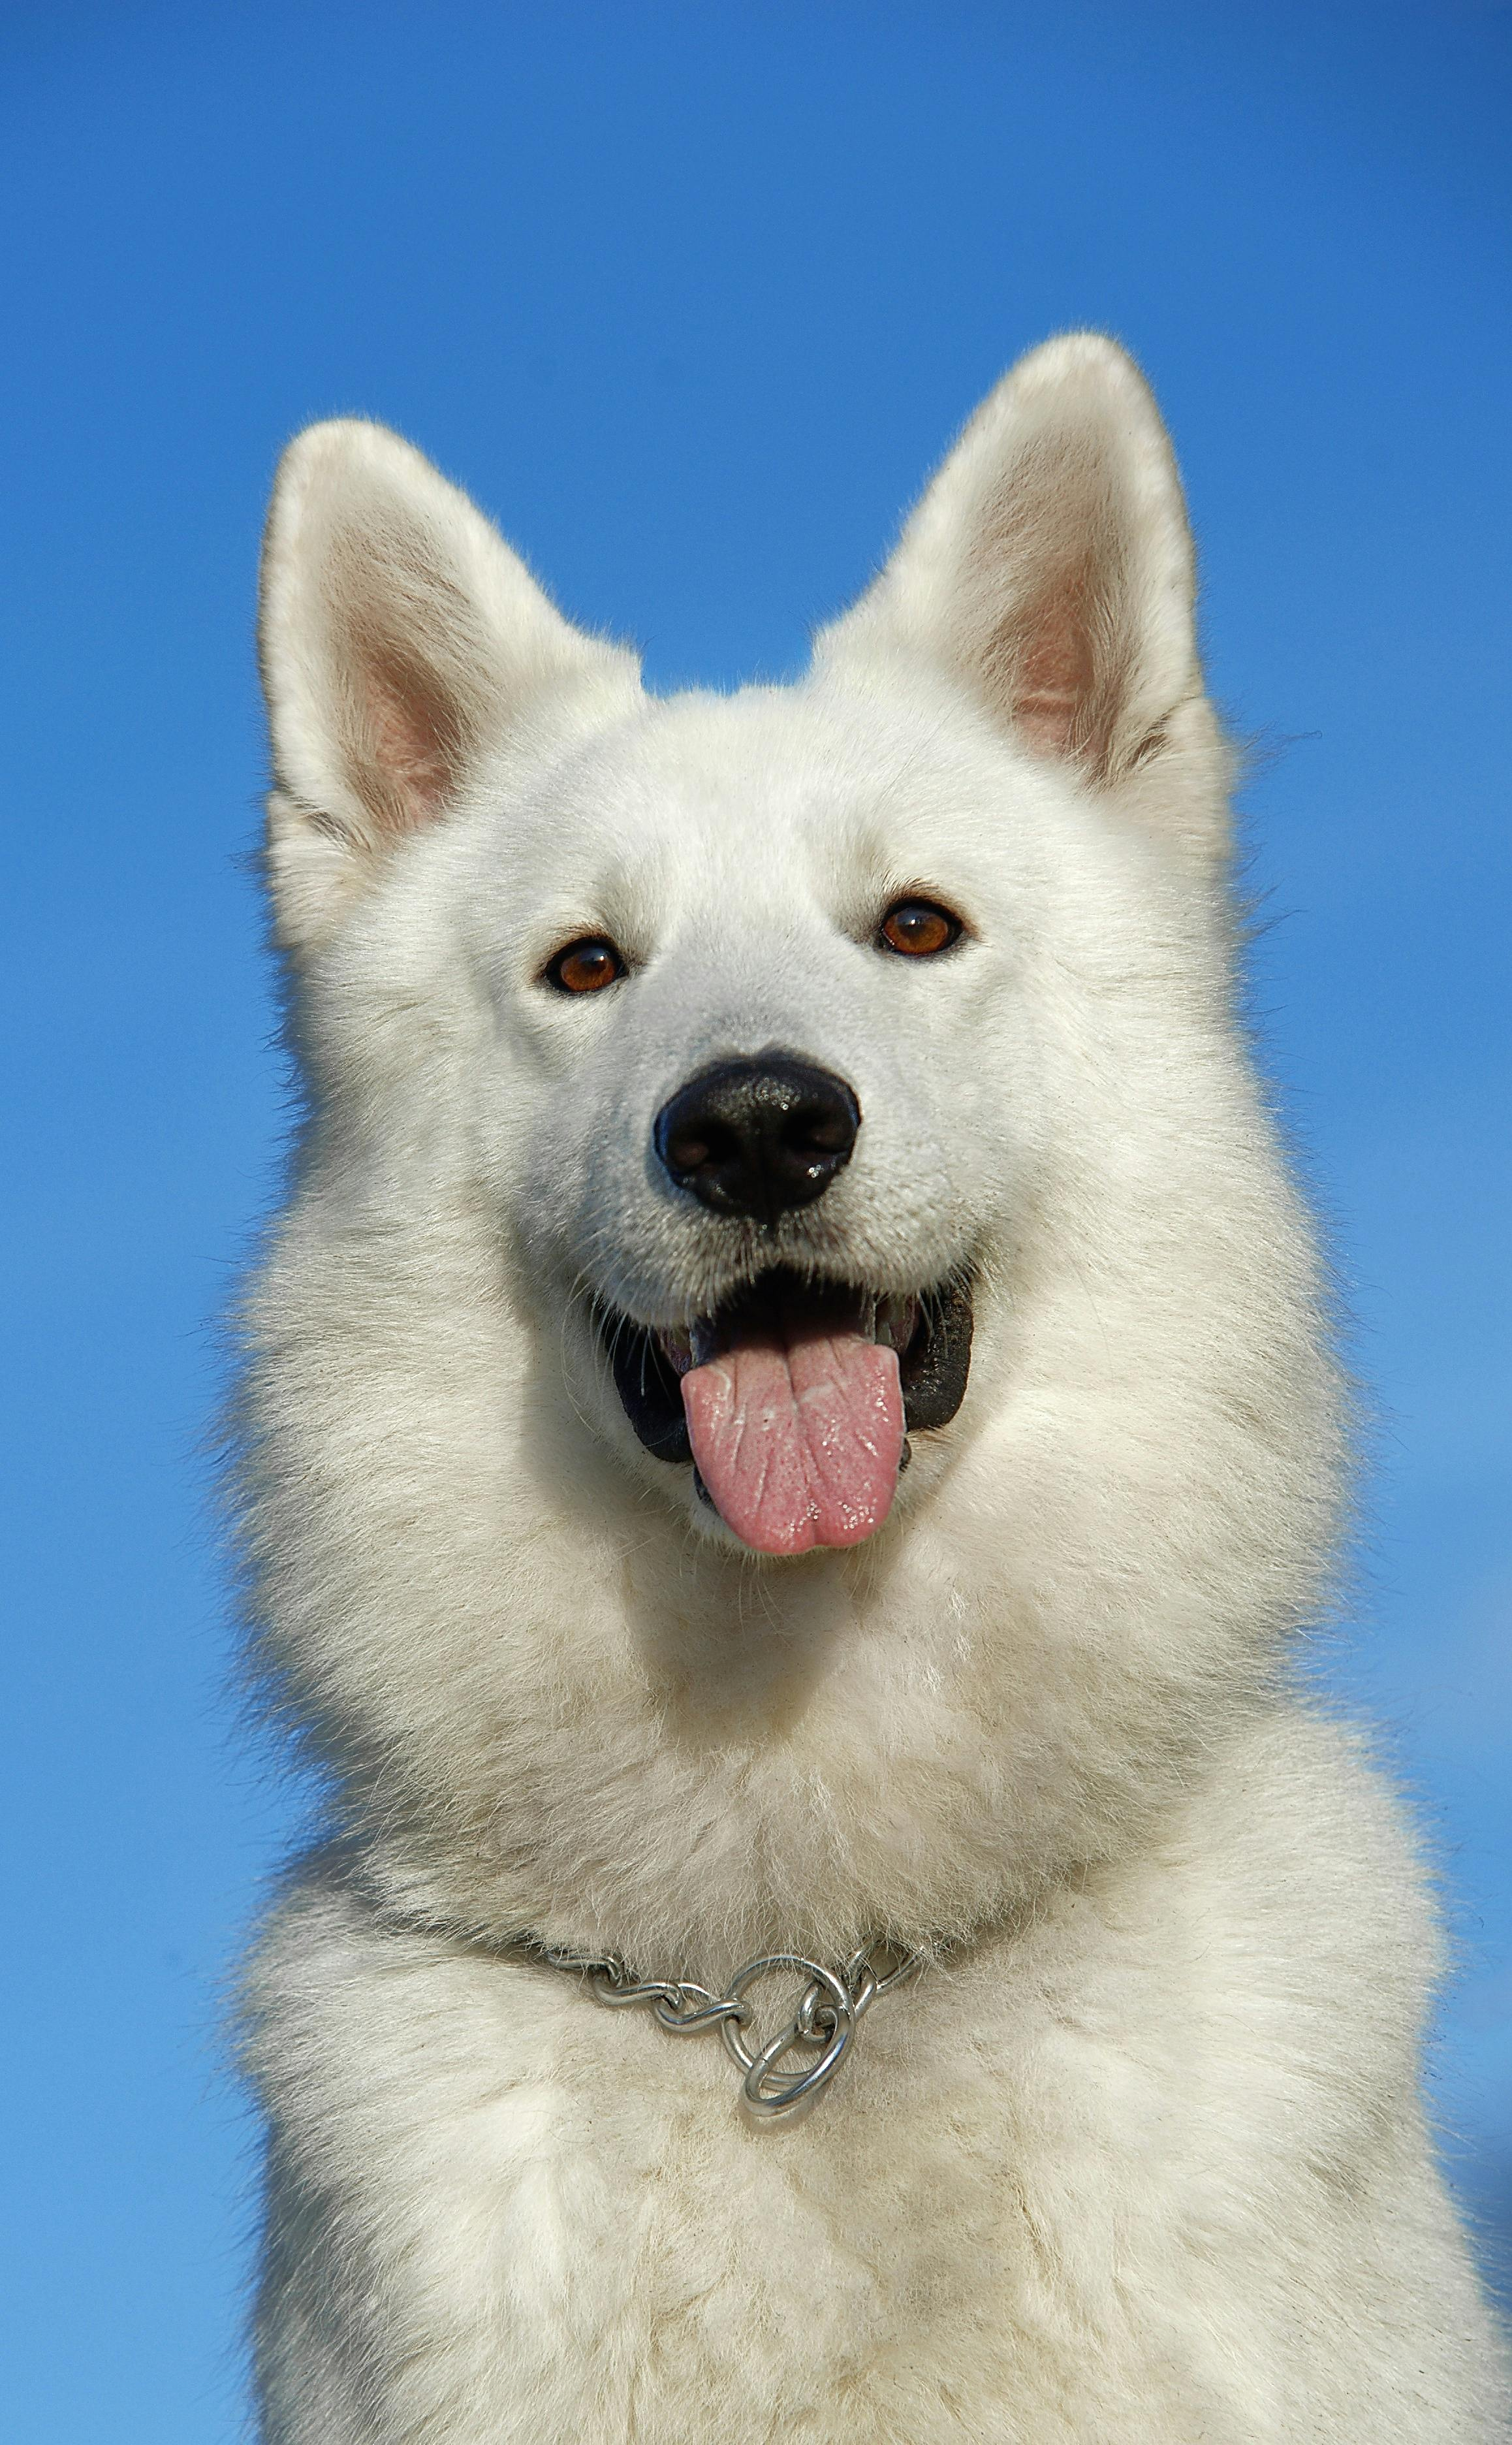
\includegraphics[width=.3\textwidth, trim={0, 27cm, 0, 18cm}, clip]{./imgs/dog.jpg}
			};
		\draw[-{Triangle[width=30pt,length=20pt]}, line width=10pt, color=desyblue](2,0) -- (4, 0);	
		\draw[line width=5pt, color=red](2,-.5) -- (4, .5);	
		\end{tikzpicture}
		\captionof{figure}{A cat is not a dog}
	\end{center}
	\LipsumPar{66}
	\begin{center}
		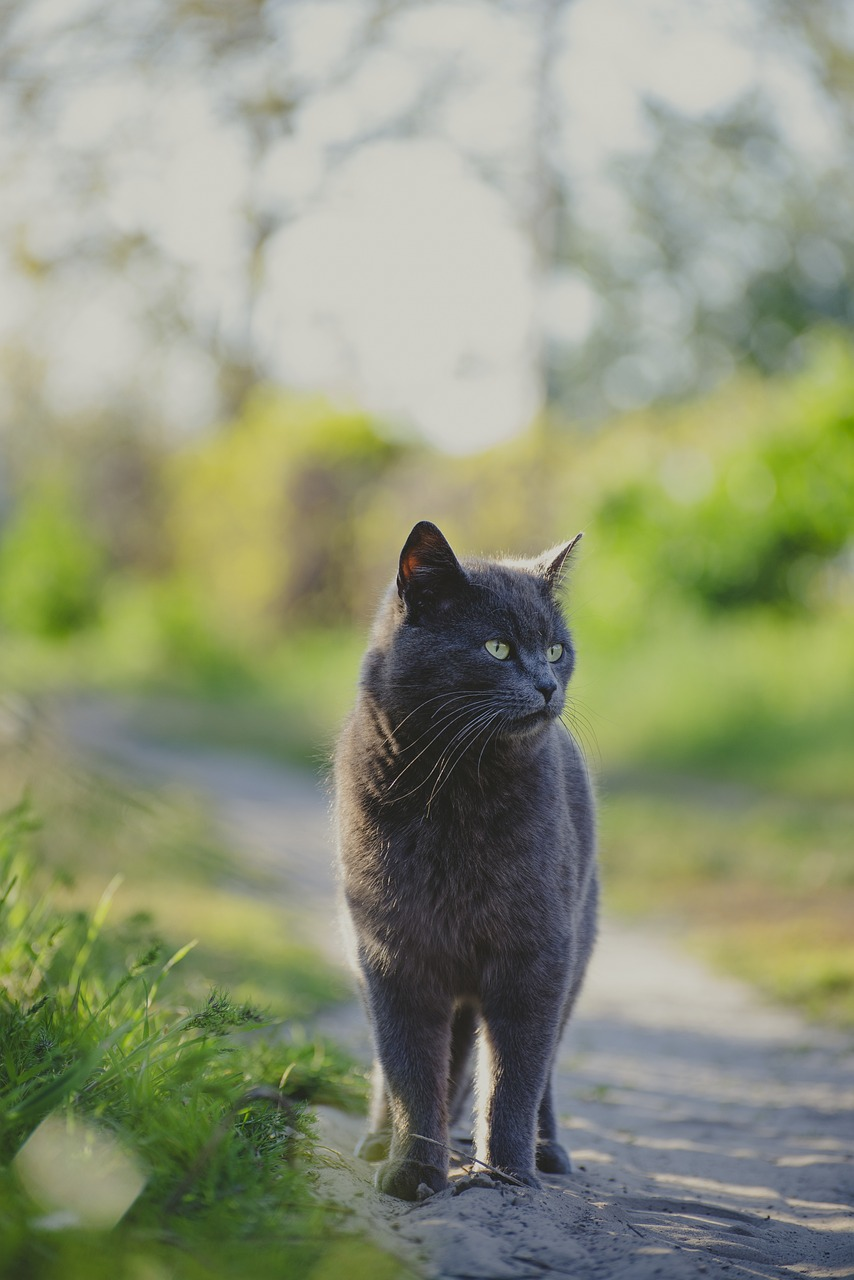
\includegraphics[width=.72\linewidth]{./imgs/cat_vertical.jpg}
		\captionof{figure}{A photo of a cute cat (I run out of ideas for things to add)}
	\end{center}
}